\documentclass{article}
\usepackage{amsmath, amssymb, graphicx}
\usepackage{hyperref}
\usepackage{geometry}
\usepackage{amsmath, amssymb, graphicx, caption}
\usepackage{hyperref}
\usepackage{listings}
\usepackage{xcolor}
\usepackage{float}
\usepackage{booktabs}
\usepackage{geometry}
\geometry{a4paper, margin=1in}
\lstset{
    basicstyle=\ttfamily\small,
    keywordstyle=\color{blue},
    commentstyle=\color{green!60!black},
    stringstyle=\color{red},
    numbers=left,
    numberstyle=\tiny\color{gray},
    stepnumber=1,
    numbersep=10pt,
    breaklines=true,
    breakatwhitespace=false,
    tabsize=4,
    frame=single,
    backgroundcolor=\color{gray!10},
    rulecolor=\color{black!20}
}

\title{Time-Varying Graphical Lasso: Summary and Application}
\author{
\begin{tabular}{cc}
Alaa Bouattour & Rayen Ben Hassen \\
Mahdi Ben Ayed & Ola Hamad \\
\end{tabular}
}
\date{}

\begin{document}

\maketitle

\tableofcontents
\newpage

\section{Article Summarization and Theoretical Formulation}
\label{sec:summary_theory}

\subsection{Introduction}
\label{subsec:intro}

In many applications, such as finance, neuroscience, and social networks, relationships between variables evolve over time. Modeling these dynamics is critical for understanding and predicting system behavior. The \textbf{Time-Varying Graphical Lasso (TVGL)} extends the classical Graphical Lasso to infer sparse precision matrices (inverse covariance matrices) that vary smoothly over time. This allows for the simultaneous discovery of network structures and their temporal evolution.

\vspace{0.5em}
\noindent\textbf{Motivation and Setting:}
\begin{itemize}
    \item Standard Graphical Lasso assumes data are independent and identically distributed (i.i.d.) and estimates a single sparse precision matrix $\Theta$.
    \item In time-dependent settings, relationships among variables evolve, requiring a framework that captures temporal variations while preserving sparsity.
    \item TVGL addresses this by introducing temporal penalties to encourage smooth transitions in precision matrices.
\end{itemize}

\vspace{0.5em}
\noindent\textbf{Applications:}
\begin{itemize}
    \item \textit{Finance}: Evolving correlations among stocks under changing market conditions.
    \item \textit{Neuroscience}: Brain connectivity changes with cognitive tasks or disease progression.
    \item \textit{Social Networks}: Shifting user interactions over time.
\end{itemize}

\subsection{Theoretical Importance of the Inverse Covariance Matrix}
\label{subsec:importance_inverse_cov}

The inverse covariance matrix, also known as the precision matrix, plays a crucial role in understanding the relationships among variables in multivariate data. It encodes the conditional independence structure of the variables:

\vspace{0.5em}
\noindent\textbf{Conditional Independence:}
If the $(i,j)$-th entry of the precision matrix $\Theta = \Sigma^{-1}$ is zero, i.e., $\Theta_{ij} = 0$, then the variables $X_i$ and $X_j$ are conditionally independent given all other variables in the system. Mathematically,
\begin{equation}
    \Theta_{ij} = 0 \quad \iff \quad P(X_i, X_j | X_{\backslash \{i,j\}}) = P(X_i | X_{\backslash \{i,j\}}) P(X_j | X_{\backslash \{i,j\}}).
\end{equation}
This makes the precision matrix a critical tool for understanding and visualizing dependencies in a network.

\vspace{0.5em}
\noindent\textbf{Proof:}
Given a multivariate Gaussian distribution $X \sim \mathcal{N}(\mu, \Sigma)$, the joint density is:
\begin{equation}
    f_X(x) = \frac{1}{(2\pi)^{p/2} |\Sigma|^{1/2}} \exp\left(-\frac{1}{2}(x - \mu)^T \Sigma^{-1} (x - \mu)\right).
\end{equation}
The conditional density of $X_i$ given $X_{\backslash i}$ can be derived from the joint Gaussian density. The conditional independence between $X_i$ and $X_j$ given $X_{\backslash \{i,j\}}$ follows directly from the structure of $\Sigma^{-1}$:
\begin{itemize}
    \item If $\Theta_{ij} = 0$, the $(i,j)$ entry in the inverse covariance matrix, this implies that there is no direct dependency between $X_i$ and $X_j$ when conditioned on the remaining variables.
    \item This property simplifies network interpretation by representing the dependencies through the graph encoded by $\Theta$.
\end{itemize}

\vspace{0.5em}
\noindent\textbf{Real-World Implications:}
In practice, this property of the precision matrix is used in:
\begin{itemize}
    \item \textit{Neuroscience:} Identifying functional connectivity in the brain by analyzing relationships between different regions over time.
    \item \textit{Finance:} Understanding dependencies between assets and mitigating risk by identifying conditional independencies.
    \item \textit{Genomics:} Mapping gene interactions by inferring sparse dependencies between genes.
\end{itemize}

\subsection{Theoretical Formulation}
\label{subsec:theory}

\subsubsection{Problem Definition and Objective}
Given a sequence of empirical covariance matrices $\{S_t\}_{t=1}^T$ computed from time-dependent data, the goal is to estimate precision matrices $\{\Theta_t\}_{t=1}^T$ for each time step $t$. The objective combines likelihood-based data fidelity, sparsity, and temporal smoothness:

\begin{equation}
\min_{\Theta_1, \ldots, \Theta_T \succ 0} \quad \sum_{t=1}^T \Big[-n_t \log \det(\Theta_t) + n_t \mathrm{Tr}(S_t \Theta_t) \Big] + \lambda \sum_{t=1}^T \|\Theta_t\|_{\text{offdiag},1} + \beta \sum_{t=2}^T \psi(\Theta_t - \Theta_{t-1}),
\end{equation}

where:
\begin{itemize}
    \item $-n_t \log \det(\Theta_t) + n_t \mathrm{Tr}(S_t \Theta_t)$: Negative log-likelihood for Gaussian data.
    \item $\|\Theta_t\|_{\text{offdiag},1}$: Encourages sparsity by penalizing off-diagonal elements.
    \item $\psi(\cdot)$: Temporal penalty encouraging smooth transitions between consecutive matrices.
    \item $\lambda, \beta$: Regularization parameters controlling sparsity and smoothness.
\end{itemize}

\subsubsection{Choices for Temporal Penalty $\psi$}
Different penalties model various evolutionary patterns:
\begin{itemize}
    \item \textbf{Element-wise L1}: $\psi(X) = \|X\|_1$ for sparse edge changes.
    \item \textbf{Group Lasso (L2)}: $\psi(X) = \sum_j \|X_{:,j}\|_2$, enforcing node-wise changes.
    \item \textbf{Laplacian}: $\psi(X) = \|X\|_F^2$, favoring smooth variations.
    \item \textbf{Infinity Norm}: $\psi(X) = \|X\|_{\infty}$ for block-wise changes.
    \item \textbf{Perturbed Node}: A row-column overlap norm allowing single-node rewiring.
\end{itemize}

\vspace{0.5em}
\noindent\textbf{Advantages of Temporal Penalties:}
\begin{itemize}
    \item \textbf{Sparsity}: Ensures the precision matrices are interpretable by promoting zero elements.
    \item \textbf{Smooth Transitions}: Captures gradual changes in relationships, reflecting real-world dynamics.
    \item \textbf{Flexibility}: Different penalties allow modeling various types of network evolution.
\end{itemize}

\subsection{Optimization Approach}
\label{subsec:optimization}

The TVGL optimization problem can be solved using:
\begin{itemize}
    \item \textbf{Interior-point methods}: Effective for small-scale problems.
    \item \textbf{First-order methods (e.g., ADMM)}: Scalable for large $p$ or $T$ by solving subproblems iteratively.
\end{itemize}

\vspace{0.5em}
\noindent\textbf{ADMM-based Approach:}
\begin{itemize}
    \item Splits the problem into smaller subproblems for each $\Theta_t$ and temporal penalty term.
    \item Ensures convergence to the global optimum with computational efficiency.
    \item Adapts well to high-dimensional settings by leveraging sparsity.
\end{itemize}

\vspace{0.5em}
\noindent\textbf{Challenges:}
\begin{itemize}
    \item High computational cost for large $T$ or $p$.
    \item Balancing sparsity and smoothness parameters ($\lambda$, $\beta$) requires careful tuning.
\end{itemize}



\section{Implementation Details and Testing on Synthetic Data}
\label{sec:implementation_synthetic}
\subsection{Implementation Details}
\label{subsec:Implementation Details}


In this section, we describe the approach taken to solve the time-varying graphical lasso (TVGL) problem. 
Since our problem dimension is of moderate size (both in terms of the number of variables $p$ 
and the number of time steps $T$), we formulate the entire problem---including the log-determinant likelihood term, 
the $\ell_1$ sparsity penalties, and the temporal smoothness penalties---as a single convex program. 
We then use CVXPY to express all constraints (particularly the positive-semidefinite constraint on $\Theta_i$) 
and rely on the \texttt{SCS} solver to handle the exponential cone representation of $\log\det(\Theta_i)$. 

The solver \texttt{SCS} is a first-order method. 
Although it can be slower or less precise than specialized interior-point methods, 
it works out of the box for exponential cone constraints, enabling us to solve $\log\det(\Theta)$ problems. 

\vspace{1em}
\noindent
\textbf{Features and Extensions:}
\begin{itemize}
    \item \emph{Multiple Smoothness Penalties} -- We can specify different $\psi(\Theta_i - \Theta_{i-1})$ functions, 
          such as element-wise $L_1$ penalties or the ``perturbed node'' penalty, simply by returning the corresponding 
          CVXPY expression (plus any auxiliary constraints).
    \item \emph{Hyperparameter Tuning} -- The parameters $\lambda$ (sparsity) and $\beta$ (smoothness) 
          can be chosen via cross-validation or other model selection criteria such Akaike Information Criterion (AIC) to balance within-timestep fit and 
          across-timestep regularity.
    \item \emph{Scalability} -- For larger problems, a block-coordinate or ADMM approach might outperform 
          a single-shot conic solve, but that is beyond our current scope.
\end{itemize}



\subsection{Synthetic Data Generation: Market Dynamics and Conditional Independence}
\label{subsec:synthetic_data}

\subsubsection{Objective}
The synthetic data aims to simulate market-like dynamics with two groups of stocks and their associated indices. The primary goal is to analyze conditional independence relationships, introduce a market event that shifts these dynamics, and test the ability of TVGL to estimate the evolving precision matrices.

\subsubsection{Setup and Dynamics}
\paragraph{Initial Configuration}
\begin{itemize}
    \item \textbf{Groups and Variables:}
    \begin{itemize}
        \item \textbf{Group 1:} 3 stocks and 1 index associated with these stocks.
        \item \textbf{Group 2:} 2 stocks and 1 index associated with these stocks.
    \end{itemize}

    \begin{figure}[h!]
    \centering
    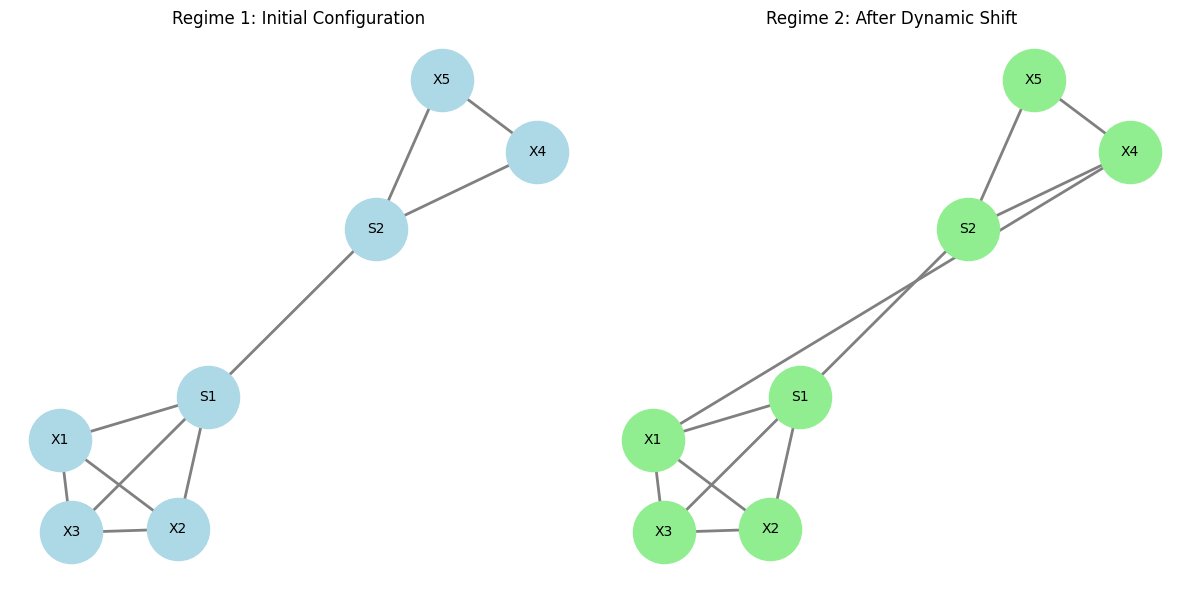
\includegraphics[width=\textwidth]{synthetic_data.png}
    \caption{Your caption here}
    \label{fig:label}
\end{figure}


    \item \textbf{Dynamic Relationships:}
    \begin{itemize}
        \item \textbf{Indexes:} Correlated and conditionally correlated. Knowing one index provides additional information about the other.
        \item \textbf{Stocks within a group:} Correlated and conditionally correlated. Knowing one stock provides information about others in the same group.
        \item \textbf{Stocks between groups:} Conditionally independent. Stocks in different groups are independent given the indices and other stocks in their respective groups.
    \end{itemize}
    \item \textbf{Matrix Constraints:}
    \begin{itemize}
        \item Precision matrix (inverse covariance matrix) reflects the dynamics, including zeros for conditional independence.
        \item Must be positive definite for invertibility.
    \end{itemize}
\end{itemize}

\paragraph{Market Change: Partial Acquisition Scenario}
\begin{itemize}
    \item \textbf{Dynamic Shift:} Partial acquisition between Group 1 and Group 2 changes the dynamics.
    \begin{itemize}
        \item Stocks in the two groups are no longer conditionally independent.
        \item Knowing a stock in one group provides additional information about stocks in the other group.
    \end{itemize}
    \item \textbf{Matrix Adjustment:}
    \begin{itemize}
        \item Update the precision matrix: Add non-zero coefficients for newly dependent variables.
        \item Ensure no changes to other zero coefficients to preserve the original conditional independence relationships.
        \item Maintain positive definiteness to ensure invertibility.
    \end{itemize}
\end{itemize}

\subsection{Implementation Plan}
\label{subsec:implementation_plan}

\paragraph{Step 1: Generate Initial Precision Matrix}
Construct the precision matrix to reflect the initial relationships:
\begin{itemize}
    \item Correlations between stocks and indexes within the same group.
    \item Conditional independence between groups.
\end{itemize}
Ensure positive definiteness of the precision matrix.

\paragraph{Step 2: Compute Covariance Matrix}
Compute the covariance matrix analytically as the inverse of the precision matrix.

\paragraph{Step 3: Generate Synthetic Data}
Use the covariance matrix to generate multivariate normal data for time horizon $T$.

\paragraph{Step 4: Modify Precision Matrix}
Adjust the precision matrix to reflect the new market dynamics:
\begin{itemize}
    \item Add non-zero coefficients for newly dependent variables.
    \item Preserve zero coefficients that correspond to conditional independence.
    \item Ensure the matrix remains positive definite and invertible.
\end{itemize}

\paragraph{Step 5: Generate Data for Updated Dynamics}
Compute the updated covariance matrix. Generate synthetic data for horizon $T'$.

\paragraph{Step 6: Concatenate Data and Estimate Relationships}
Concatenate data from the two horizons. Estimate the covariance matrices for both regimes using the synthetic data. Compute the precision matrices from the estimated covariance matrices.

\paragraph{Step 7: Analyze Results}
Identify pairs of variables that are conditionally independent in each regime. Compare the results to the theoretical precision matrices and highlight discrepancies where estimation produces incorrect results.

\subsection{Testing and Results}

To test the correctness and robustness of the algorithm, we created two datasets based on the principles previously discussed. Both datasets are derived from two true inverse covariance matrices.

\textbf{Matrix 1:}
\[
K_1 = \begin{bmatrix}
2.0 & 0.2 & 0.2 & 0.3 & 0.0 & 0.0 & 0.0 \\
0.2 & 2.0 & 0.2 & 0.3 & 0.0 & 0.0 & 0.0 \\
0.2 & 0.2 & 2.0 & 0.3 & 0.0 & 0.0 & 0.0 \\
0.3 & 0.3 & 0.3 & 2.0 & 0.0 & 0.0 & 0.2 \\
0.0 & 0.0 & 0.0 & 0.0 & 2.0 & 0.2 & 0.3 \\
0.0 & 0.0 & 0.0 & 0.0 & 0.2 & 2.0 & 0.3 \\
0.0 & 0.0 & 0.0 & 0.2 & 0.3 & 0.3 & 2.0 \\
\end{bmatrix}
\]

\textbf{Matrix 2:}
\[
K_2 = \begin{bmatrix}
2.0 & 0.2 & 0.2 & 0.3 & 0.3 & 0.0 & 0.0 \\
0.2 & 2.0 & 0.2 & 0.3 & 0.0 & 0.0 & 0.0 \\
0.2 & 0.2 & 2.0 & 0.3 & 0.0 & 0.0 & 0.0 \\
0.3 & 0.3 & 0.3 & 2.0 & 0.0 & 0.0 & 0.2 \\
0.3 & 0.0 & 0.0 & 0.0 & 2.0 & 0.2 & 0.3 \\
0.0 & 0.0 & 0.0 & 0.0 & 0.2 & 2.0 & 0.3 \\
0.0 & 0.0 & 0.0 & 0.2 & 0.3 & 0.3 & 2.0 \\
\end{bmatrix}
\]

\subsubsection{First Dataset: True Permanent Change}
The first dataset represents a true permanent change in the market dynamics between two specific nodes. We generated 80,000 historical points from \(K_1\) followed by 120,000 points from \(K_2\). To align with the methodology, we consider each 20,000 points as one period. Therefore, the vector of true periods is:
\[
[K_1, K_1, K_1, K_1, K_2, K_2, K_2, K_2, K_2, K_2]
\]
We expect a change in the estimated covariance matrix between the 4th and 5th periods. The testing code details can be found in the \texttt{synthetic_data_generatinon_and_testing.ipynb} notebook.

\begin{figure}[h!]
    \centering
    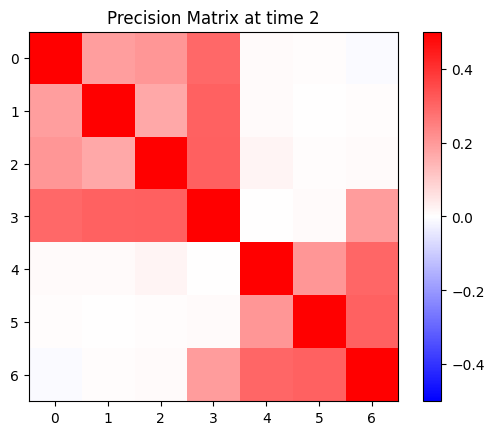
\includegraphics[width=0.22\textwidth]{matrix1.png}
    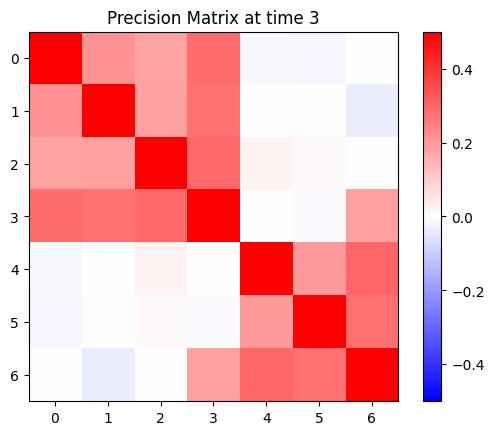
\includegraphics[width=0.22\textwidth]{matrix2.png}
    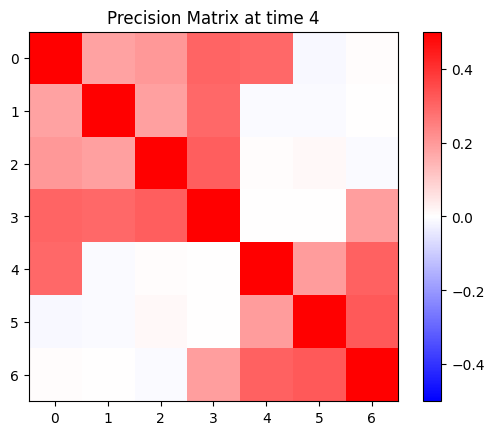
\includegraphics[width=0.22\textwidth]{matrix3.png}
    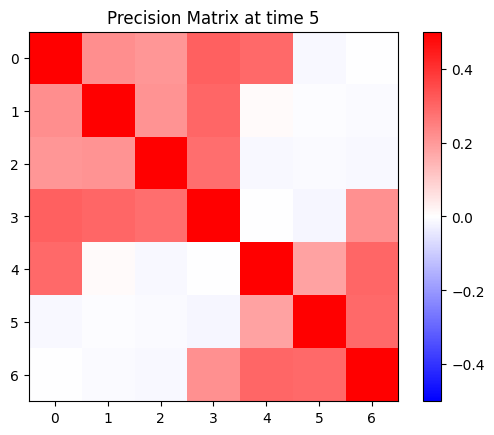
\includegraphics[width=0.22\textwidth]{matrix4.png}
    \caption{Estimated Matrices for True Permanent Change}
\end{figure}
\newpage
\begin{figure}[h!]
    \centering
    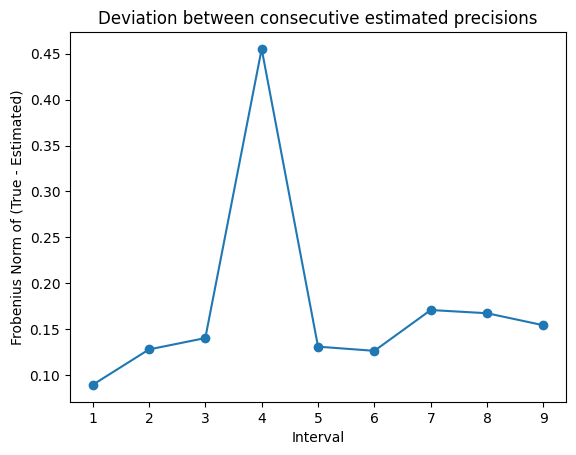
\includegraphics[width=0.45\textwidth]{difference1.png}
    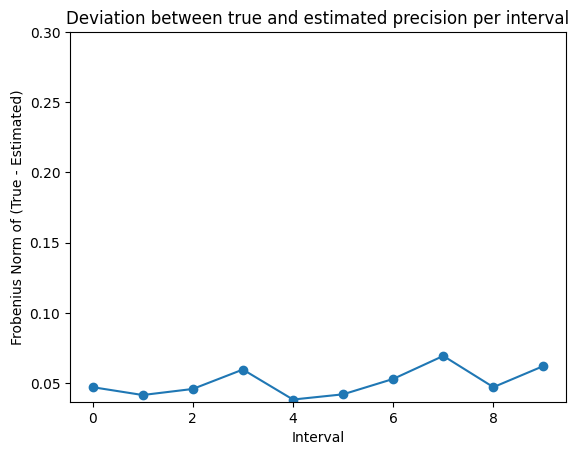
\includegraphics[width=0.45\textwidth]{difference2.png}
    \caption{Difference Between True and Estimated Matrices}
\end{figure}

We observe that the estimated matrices are very close to the true matrices, with a difference in norm around 8\% for all matrices. Additionally, we notice a peak in the curve of \(\|\Theta(i) - \Theta(i-1)\|\) at the 5th period, indicating a change in market dynamics. This aligns with real-world scenarios where such changes signify significant market shifts.

\subsubsection{Second Dataset: Temporary Perturbation}
The second dataset represents a temporary perturbation in market dynamics. Here, one period (20,000 points) is governed by \(K_2\), while all other periods follow \(K_1\). The vector of true periods is:
\[
[K_1, K_1, K_1, K_1, K_2, K_1, K_1, K_1, K_1, K_1]
\]
In this case, we expect the system to be robust to this noise and maintain a consistent matrix structure.

\begin{figure}[h!]
    \centering
    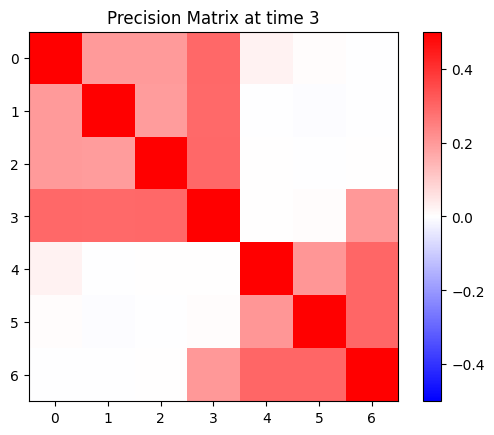
\includegraphics[width=0.22\textwidth]{amatrix1.png}
    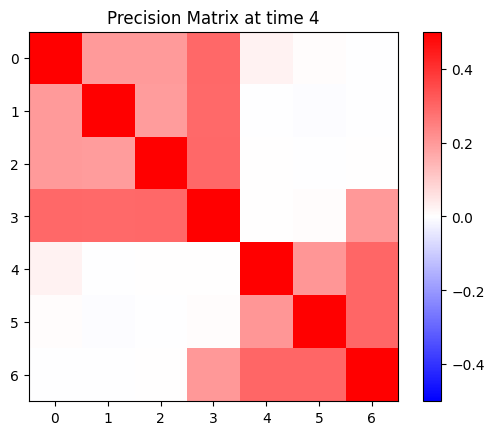
\includegraphics[width=0.22\textwidth]{amatrix2.png}
    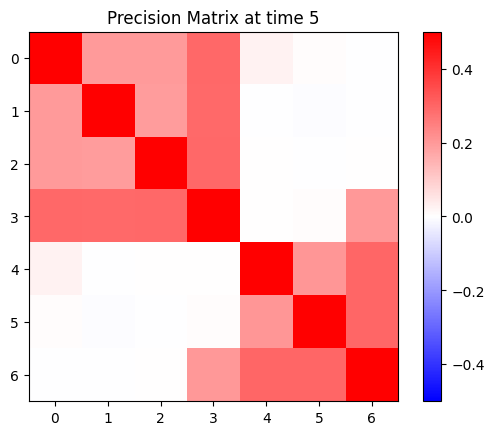
\includegraphics[width=0.22\textwidth]{amatrix3.png}
    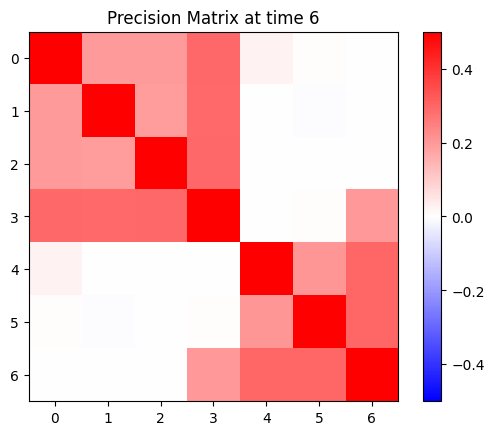
\includegraphics[width=0.22\textwidth]{amatrix4.png}
    \caption{Estimated Matrices for Temporary Perturbation}
\end{figure}
\newpage
\begin{figure}[h!]
    \centering
    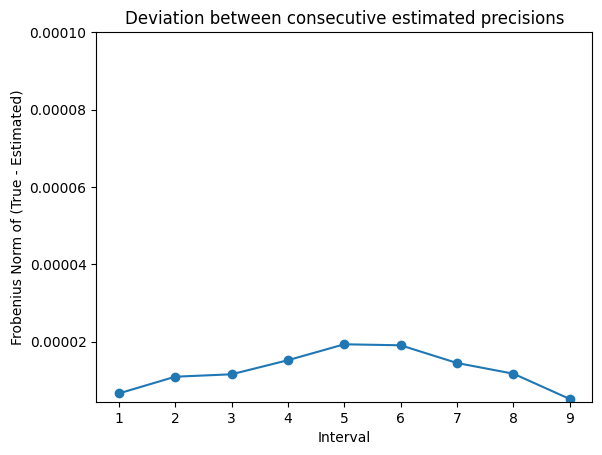
\includegraphics[width=0.45\textwidth]{adifference1.png}
    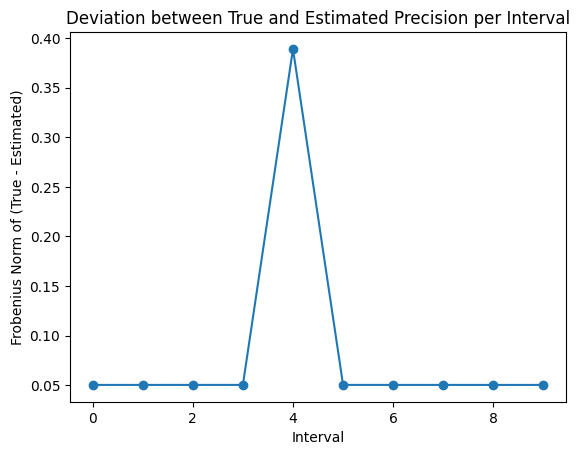
\includegraphics[width=0.45\textwidth]{adifference2.png}
    \caption{Difference Between True and Estimated Matrices for Temporary Perturbation}
\end{figure}

We observe that the estimated matrices remain consistent apart from the temporary perturbation in the 5th period. Moreover, the curve of \(\|\Theta(i) - \Theta(i-1)\|\) remains stable, effectively avoiding a false detection of market changes. This demonstrates the system's robustness to noise in real-world scenarios.

 \section{Event detection: S\&P500 case}


\subsection{Overview}
By examining historical stock prices, we can infer a financial network to model relationships between different companies. Learning the structure of this network is useful because it allows us to model how certain stocks are related. This can be leveraged to predict future prices, understand economic trends, or diversify a portfolio by avoiding highly correlated stocks. In this study, we infer this network by treating the daily closing price of each stock as a sensor observation and applying the TVGL framework to identify structural changes.

\subsection{Single-Stock Perturbations}
To detect localized events, we observed daily stock prices for six large American companies: Apple, Google, Amazon, Intel, Boeing, and FedEx. Generally, large companies exhibit a stable correlation network; however, sudden events can cause shifts in this structure. The TVGL model allows for the detection of such events by incorporating a temporal dynamic that penalizes changes affecting single nodes. This approach reflects situations where a specific company experiences a significant perturbation, leaving the rest of the network relatively unchanged. By solving the TVGL optimization problem with this node-perturbation penalty, we identified one major event during the dataset's time period, which corresponded to a significant shift in Apple's connections. Further investigation revealed that this event coincided with Apple's announcement of the original iPad.

\subsection{Large-Scale Events}
 Beyond single-stock perturbations, the TVGL framework can be extended to detect macro-level events affecting the entire market. By applying the model to the S\&P 500 dataset, we analyzed structural shifts in the network of the 6 major companies. The maximum temporal deviation, identified through an $\ell_1$ penalty, corresponded to the period April-Mai 2010. This period aligns with the infamous "Flash Crash," during which the market experienced a sudden and dramatic drop of 9\% before quickly rebounding. 

\subsection{Results}
The deviations between consecutive precision matrices were plotted to detect significant events. A peak in the deviation plot indicates a potential event. As shown in Figure \ref{fig:deviation}, a significant deviation occurred around mid-December 2009/ January 2010, suggesting a structural change in the covariance structure of stock returns (the single-stock perturbation example). Another significant deviation occured around April/Mai 2010, which consistent with the "Flash Crash" (Large-Scale events example).

\begin{figure}[h!]
    \centering
    \includegraphics[width=0.6\textwidth]{output.png}
    \caption{Deviation between True and Estimated Precision per Interval}
    \label{fig:deviation}
\end{figure}


\section{Trading Strategy Comparison: Inverse Covariance vs. Time-Varying Graphical Lasso (TVGL)}

\subsection{Overview}

In portfolio optimization, accurately estimating the precision matrix, which is the inverse of the covariance matrix, is crucial for determining optimal asset weights. Two prevalent methods for precision matrix estimation are the traditional Inverse Covariance approach and the Time-Varying Graphical Lasso (TVGL). This section presents a comparative analysis of these two methods within a trading strategy framework, highlighting their performance based on cumulative returns, Sharpe Ratios, and Maximum Drawdowns.

\subsection{Methodology}

\subsubsection{Data Acquisition and Preparation}

The dataset comprises daily adjusted closing prices for six major stocks: Apple Inc. (\texttt{AAPL}), Alphabet Inc. (\texttt{GOOG}), Amazon.com Inc. (\texttt{AMZN}), Intel Corporation (\texttt{INTC}), The Boeing Company (\texttt{BA}), and FedEx Corporation (\texttt{FDX}). The data spans from August 1, 2010, to August 1, 2015.

\begin{itemize}
    \item \textbf{Data Source}: Yahoo Finance via the \texttt{yfinance} library.
    \item \textbf{Return Calculation}: Daily returns are computed as percentage changes of the adjusted closing prices.

\end{itemize}

\subsubsection{Precision Matrix Estimation Methods}

\paragraph{1. Inverse Covariance}

The Inverse Covariance method involves calculating the empirical covariance matrix of asset returns over a rolling window and then inverting it to obtain the precision matrix. A small regularization term (\(\lambda = 10^{-4}\)) is added to the diagonal of the covariance matrix to ensure numerical stability and invertibility.


\[
\mathbf{\Theta} = \left( S + \lambda \mathbf{I} \right)^{-1}
\]

To calculate this matrix, we used a window of 25 trading days. So, \( S \) in the above equation is the covariance matrix for the period of 25 days, and \( \Theta \) is our approximation of the inverse of the covariance matrix.

\paragraph{2. Time-Varying Graphical Lasso (TVGL)}

TVGL extends the graphical lasso by allowing the precision matrix to evolve over time, capturing temporal dependencies and structural changes in the asset relationships. The method estimates a sequence of precision matrices (\(\mathbf{\Theta}_t\)) over overlapping data segments, enforcing sparsity and smoothness through regularization parameters \(\lambda\) and \(\beta\).

\[
\mathbf{\Theta}_t = \arg\min_{\mathbf{\Theta}} \left\{ -\log \det(\mathbf{\Theta}) + \text{trace}(\mathbf{\Sigma}_t \mathbf{\Theta}) + \lambda \|\mathbf{\Theta}\|_1 + \beta \|\mathbf{\Theta}_t - \mathbf{\Theta}_{t-1}\|_F^2 \right\}
\]

The optimization problem described above is calculated over a period of 125 trading days. The duration between two consecutive \( \Theta_i \) is 25 days, consistent with the period used for the inverse covariance matrix method. The goal is to compare two comparable matrices. 

Our precision matrix, \( \Theta \), is the final \( \Theta_i \) generated in this process. The key idea is that this precision matrix should approximate the inverse covariance matrix. However, it is "regularized" and incorporates temporal evolution information of \( \Theta \) over the broader period of 125 days.

\subsubsection{Portfolio Weight Calculation}

For each precision matrix estimated, the portfolio weights are derived using the minimum variance approach:

\[
\mathbf{w} = \frac{\mathbf{\Theta} \mathbf{1}}{\mathbf{1}^\top \mathbf{\Theta} \mathbf{1}}
\]

where \(\mathbf{1}\) is a vector of ones. This ensures that the weights sum to unity, adhering to the full investment constraint.

\subsubsection{Trading Strategy Execution}

The trading strategy operates as follows:

\begin{enumerate}
    \item \textbf{Rolling Window}: Starting from the \texttt{test\_date} (day 251), the strategy uses a rolling window of past returns (\texttt{window\_size}) to estimate the precision matrix ((\texttt{window\_size}) is 25 days for the Inverse Covariance method and is 125 days for TVGL method). 
    \item \textbf{Weight Allocation}: Based on the estimated precision matrix, portfolio weights are calculated.
    \item \textbf{Return Calculation}: These weights are applied to the subsequent \texttt{step\_size}=25 days to compute portfolio returns by compounding daily returns.
    \item \textbf{Iteration}: The window slides forward by \texttt{step\_size} days, and the process repeats until the end of the dataset.
\end{enumerate}

\subsection{Results}

The performance of the two precision matrix estimation methods is summarized in Table \ref{tab:performance}.

\begin{table}[H]
    \centering
    \caption{Performance Metrics Comparison}
    \label{tab:performance}
    \begin{tabular}{lccc}
        \toprule
        \textbf{Method} & \textbf{Cumulative Return} & \textbf{Sharpe Ratio} & \textbf{Maximum Drawdown} \\
        \midrule
        Inverse Covariance & 1.429987 & 1.703372 & 0.080481 \\
        TVGL               & 1.737669 & 1.878408 & 0.098915 \\
        \bottomrule
    \end{tabular}
\end{table}

\subsubsection{Interpretation of Metrics}

\paragraph{1. Cumulative Return}

\begin{itemize}
    \item \textbf{Inverse Covariance}: A cumulative return of 1.429987 indicates a 142.9987\% return over the backtesting period.
    \item \textbf{TVGL}: A cumulative return of 1.737669 signifies a 173.7669\% return, outperforming the Inverse Covariance method.
\end{itemize}

\paragraph{2. Sharpe Ratio}

The Sharpe Ratio measures risk-adjusted returns. Values above 1 are considered good, with higher values indicating better performance relative to risk.

\begin{itemize}
    \item \textbf{Inverse Covariance}: 1.703372
    \item \textbf{TVGL}: 1.878408
\end{itemize}

Both methods exhibit strong Sharpe Ratios, with TVGL slightly outperforming Inverse Covariance.

\paragraph{3. Maximum Drawdown}

Maximum Drawdown assesses the largest peak-to-trough decline, reflecting downside risk.

\begin{itemize}
    \item \textbf{Inverse Covariance}: 0.080481 (8.0481\%)
    \item \textbf{TVGL}: 0.098915 (9.8915\%)
\end{itemize}

While TVGL achieved higher returns, it also experienced a slightly larger drawdown compared to Inverse Covariance.

\subsection{Visualization}

Figure \ref{fig:cumulative_returns} illustrates the cumulative returns over time for both methods.

\begin{figure}[H]
    \centering
    \includegraphics[width=0.8\textwidth]{output2.png}
    \caption{Cumulative Returns Comparison: Inverse Covariance vs. TVGL}
    \label{fig:cumulative_returns}
\end{figure}

\subsection{Discussion}

The comparative analysis reveals that the TVGL method outperforms the traditional Inverse Covariance approach in terms of cumulative returns and Sharpe Ratio. This suggests that TVGL's ability to capture temporal dependencies and structural changes in the asset relationships leads to more effective portfolio optimization. However, TVGL also incurs a slightly higher Maximum Drawdown, indicating increased exposure to downside risk during certain periods.

\subsubsection{Possible Reasons for TVGL's Superior Performance}

\begin{itemize}
    \item \textbf{Temporal Dynamics}: TVGL accounts for time-varying relationships among assets, allowing the model to adapt to changing market conditions more effectively than the static Inverse Covariance method.
    \item \textbf{Sparsity and Smoothness}: The regularization parameters \(\lambda\) and \(\beta\) in TVGL enforce sparsity and smooth transitions between precision matrices, enhancing the stability and interpretability of the model.
    \item \textbf{Overfitting Prevention}: By incorporating regularization, TVGL mitigates the risk of overfitting, leading to more robust out-of-sample performance.
\end{itemize}

\subsubsection{Considerations and Future Work}

While TVGL demonstrates superior performance, the slightly higher drawdown warrants further investigation. Future work could explore:

\begin{itemize}
    \item \textbf{Hyperparameter Optimization}: Fine-tuning \(\lambda\) and \(\beta\) to balance return maximization and drawdown minimization.
    \item \textbf{Inclusion of Transaction Costs}: Including transaction costs could provide a more realistic assessment of the strategy's performance.
    \item \textbf{Expanded Asset Universe}: Testing the strategy on a broader set of assets to evaluate scalability and robustness.
    \item \textbf{Alternative Portfolio Optimization Techniques}: Exploring mean-variance optimization or incorporating expected returns could enhance performance.
\end{itemize}


\end{document}


\end{document}
